\chapter{Research Testing}
To provide information about the behaviour of a quadcopter with variable pitch propellers, a series of consecutive tests are performed. The characteristics of variable pitch are compared with fixed pitch. The following tests are carried out at KONGSBERG Innovation Center in a confined area. The series of tests are performed with the same physical quadcopter to gain the most comparable datasets.  The propellers on the variable pitch quadcopter are fixated at a fixed pitch, creating the fixed pitch test object. \bigskip

Having two independent test objects who are providing two independent datasets, their outcome can be compared. Assuming that the outcome of each of the tests are independent, it is expected that the results will be normal distributed. When comparing two independent datasets, the most common method for analysis is the t-test \cite{statistikk}. The t-test is a statistical hypothesis test and it is used to test if the average value of a normalized dataset is significantly different from the null hypothesis, and if there is a significant difference between the average values in the two datasets.\bigskip

The following tests requires that a null hypothesis and an alternative hypothesis must be stated. The hypotheses are stated in such a way that they are mutually exclusive as in Eq. \ref{eq:nh}. That is, if one is true, the other must be false; and vice versa \cite{statistikk4}. $VPQ_i$ expresses the stochastic variable for the measured value $i$ for dataset 1, $n_1$. $FPQ_j$ expresses the stochastic variable for the measured value $j$ for dataset 2, $n_2$. Assuming that $VPQ_i$ is independent and normal distributed with expectation, $\mu_1$, and standard deviation, $\sigma_1$.  Assuming that $FPQ_i$ is independent and normal distributed with expectation, $\mu_2$, and standard deviation $\sigma_2$. It must also be assumed that $VPQ_i$ are independent from $FPQ_i$. 
\begin{equation}
\label{eq:nh}
H_0:\: \mu_1 = \mu_2 \quad \quad H_1:\: \mu_1 \neq \mu_2
\end{equation}

The null hypothesis is tested in the t-test. If the mean in the datasets obtained are the same, the null hypothesis is kept, according to the t-test. Otherwise, the null hypothesis is rejected and there is a difference between the two datasets. If the the null hypothesis is discarded, the difference between the datasets are statistically significant. It is therefore unlikely that the differences between datasets are due to coincidences. Statistical significance indicates the likelihood that the observed difference between the datasets are due to coincidences.
%%%%%%%%%%%%%%%%%%%%%%%%%%%%%%%%%%%%%%%
%%%%%%%%%%%%%%%%%%%%%%%%%%%%%%%%%%%%%%%
\newpage
\section{Variable Pitch Landing}
\label{sec:landtest}
To determine if a quadcopter with variable pitch propellers can land more precise than a quadcopter with fixed pitch, a series of samples must be obtained. Two sets of samples are obtained by landing the quadcopter multiple times with the two configurations, variable pitch and fixed pitch. When a number of landings have been conducted, a conclusion can be drawn. The hypotheses are:\bigskip

$H_0$ = Variable pitch propellers provide the same landing precision as fixed pitch propellers $(\mu_1 = \mu_2 )$\\
$H_1$ = Variable pitch propellers do not provide the same landing precision as fixed pitch propellers $(\mu_1 \neq \mu_2 )$\\

\subsection{\textsc{\medium Test Setup}}
In Fig. \ref{fig:landsetup} an illustration of the test setup is displayed. The quadcopter is controlled by a pilot with a Radio Controller, and all flights are tracked with the Qualisys Motion Tracking System. To obtain the most comparable data, the pilot followed the following guidelines:
\begin{enumerate}
  \item The pilot shall stand behind the rear end of the quadcopter along the y-axis, when x=0
  \item Provide throttle for lift in z-axis and hover above ground effect
  \item Move forward in y-axis until target position is reached
  \item Land the quadcopter as close to the target position as possible
\end{enumerate}\bigskip

For Qualisys to be able to capture the motion of the quadcopter, four reflective markers are mounted. One marker is mounted in the center-top of the quadcopter and this marker provides information about the distance from the target position when the quadcopter has landed. The target position in Qualisys is set at (x,y) = (0,0).

\begin{figure}[H]
    \centering
    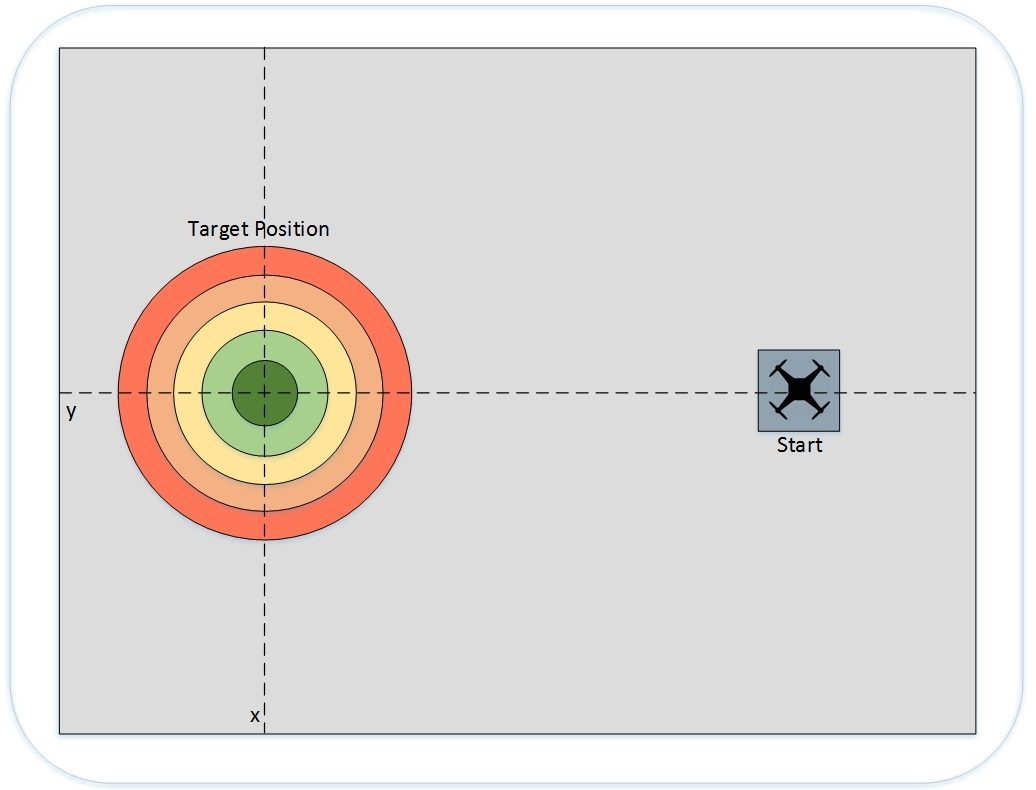
\includegraphics[width = 0.7\textwidth]{VAPIQ-PICTURES/landingtest}
    \caption{Test Setup for Landing Test}
    \label{fig:landsetup}
\end{figure}

In Tab. \ref{tab:landingdata1} the quadcopter configurations of the datasets, respectively, for all landings performed are displayed. 

\begin{table}[H]
\caption{Landings Performed}
\\
\label{tab:landingdata1}
\centering
\
\begin{tabular}{| c | c | c | c |} 
 \hline
  Quadcopter Configuration  & Dataset & Number of landings & Pilot \\
 \hline
VPQ & 1 & 20 & Tommy André Bertelsen  \\
FPQ & 1 & 20 & Tommy André Bertelsen  \\
VPQ & 2 & 51 & Tomas Lyngroth   \\
FPQ & 2 & 40 & Tomas Lyngroth  \\
\hline
\end{tabular}
\end{table}

To process the data gained, Matlab and Excel are used. In Appendix XX the Matlab script for this test is displayed and in Appendix XX the tables with all samples from the datasets can be found.

\subsection{\textsc{\medium Test Assessment}}
% [Enter a comprehensive assessment of your interpretation of how adequate the test was in light of how thorough the test plan said it should be? What wasn't tested well enough?]
%[Describe any variances between the testing that was planned and the testing that actually occurred.  Also, provide a assessment of the manner in which the test environment may be different from the operational environment and the effect of this difference on the test results
%[Provide a brief description of the unexpected results, problems, or defects that occurred during the testing.]
The quadcopter was flown in acro-mode with a radio controller. In acro-mode the pilot must compensate for every unwanted movement. To obtain comparable datasets, the same flight route must be followed. However, in acro-mode it is almost impossible to reenact the exact same route, which might inflict the data obtained in this test.   \bigskip

When the pilot maneuvers the quadcopter to the specified target, the pilots perception of the target might differ from the actual location of the target. The pilots perception might depend on the pilots position in the room and how the pilot views the target.\bigskip

In Fig. \ref{fig:landsetup2} and Fig. \ref{fig:landsetup3} the blue circles represent the actual landing position of the quadcopter. The red circles represent the calculated perceived position based on the mean of the x and y plots from the landing positions. The mean value of the x and y plots, for the respective datasets, are deducted from the actual position. This is done to remove the human error made by the pilot when he tries to meet the target position. 

\begin{figure}[H]
    \centering
    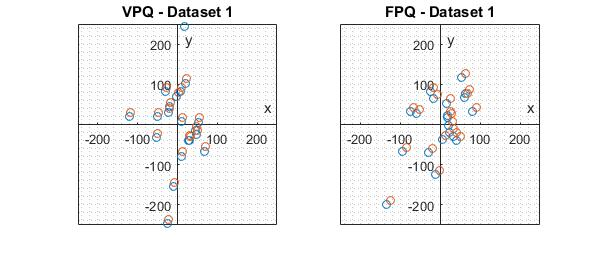
\includegraphics[width = 0.9\textwidth]{VAPIQ-PICTURES/actualvsbiased1}
    \caption{Landing Dataset 1 - Actual landing (blue) vs. landing when bias is removed (red)}
    \label{fig:landsetup2}
\end{figure}

\begin{figure}[H]
    \centering
    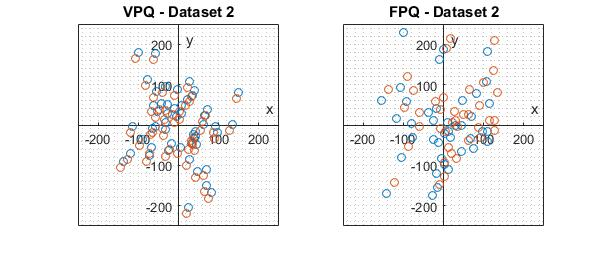
\includegraphics[width = 0.9\textwidth]{VAPIQ-PICTURES/actualvsbiased2}
    \caption{Landing Dataset 2 - Actual landing (blue) vs. landing when bias is removed (red)}
    \label{fig:landsetup3}
\end{figure}

Fig. \ref{fig:landsetup2} and Fig. \ref{fig:landsetup3} shows that the error of perception is most prominent along the y-axis for all datasets. It is seemingly logical that the error in the y-axis is the most prominent since the pilot is positioned in approximately x = 0, and therefore it is easier to perceive where the quadcopter is in the x-axis. For further calculations, the datasets where the bias is removed are used.\bigskip

From Tab. \ref{tab:landingdata1} the pilots used for the respective datasets are displayed. The difference in flight style and experience of the pilots can have an impact on the test results. Tommy André Bertelsen is a very experienced multicopter pilot, and this can also be shown in the test results. 

\subsection{\textsc{\medium Test Results}}
From Fig. \ref{fig:histo1} the histograms for the respective datasets are displayed. Fig. \ref{fig:histo1} shows that the values obtained from each dataset are approximately normal distributed. VPQ - Dataset 1 and FPQ - Dataset 1 only have 20 samples each, which makes it less likely to be normal distributed. \bigskip

The two datasets for VPQ and FPQ are added to the same plot and they become the total dataset that will be put into the t-test. Fig. \ref{fig:totalbiased} shows the total biased landing spots for VPQ and FPQ. In Fig \ref{fig:histo2} the histograms for total landings are displayed.

\begin{figure}[H]
    \centering
    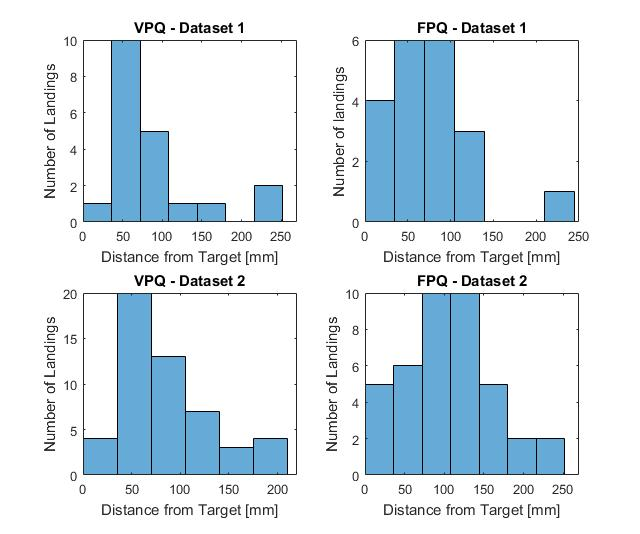
\includegraphics[width = 0.8\textwidth]{VAPIQ-PICTURES/histotomas}
    \caption{Histogram for Dataset 1 and Dataset 2}
    \label{fig:histo1}
\end{figure}

\begin{figure}[H]
    \centering
    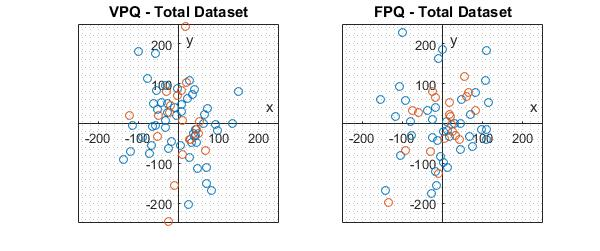
\includegraphics[width =1\textwidth]{VAPIQ-PICTURES/totalbiased}
    \caption{All captured landings when bias is removed}
    \label{fig:totalbiased}
\end{figure}

\begin{figure}[H]
    \centering
    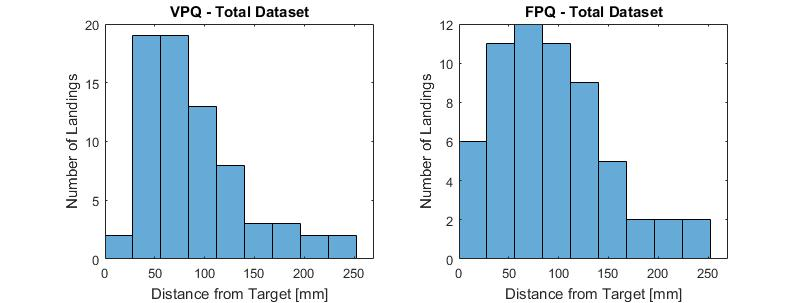
\includegraphics[width = 1\textwidth]{VAPIQ-PICTURES/histoall}
    \caption{Histogram for all captured landings}
    \label{fig:histo2}
\end{figure}

The obtained samples of data in Tab. \ref{tab:landingdata} shows the means of all datasets and the total datasets. Tab. \ref{tab:landingdata} also shows the variance and how many samples in each set of data.

\begin{table}[H]
\caption{Table of Data}
\label{tab:landingdata}
\centering
\begin{tabular}{| c | c |c| c|} 
  \hline
  Quadcopter Dataset   & Mean & Variance & Number of landings \\
 \hline
 VPQ1 & 87.82 & 3961.8   & 20\\
 FPQ1 & 78.21 & 2484.1   & 20\\
 VPQ2 & 90.44 & 2265.4   & 51\\
 FPQ2 & 102.50  & 3451.7  & 40\\
  \hline
 VPQtot & 89.13 & 2694.9   & 71\\
 FPQtot & 90.36 & 3215.0   & 60\\
 \hline
\end{tabular}
\end{table}

The similarity of the means from the two datasets are tested based on test observer T (t-test). The test observer T is determined by:\\
\begin{equation}
\label{eq:T}
  T = \frac{\overline{VPQtot} - \overline{FPQtot}}{\sqrt{\frac{S_1^2}{n_1}+\frac{S_2^2}{n_2}}} = \frac{89.13-90.36}{\sqrt{ \frac{2694.9}{71}+\frac{3215.0}{60} }} = -0.13
\end{equation}
\\
When considering whether or not the null hypothesis shall be discarded, the level of significance must be determined, based on the level of rejection error that can be accepted. It is normal to choose a level of significance, $\alpha=0.05$. \bigskip

The degrees of freedom are determined by the size of the datasets. In this case, the degrees of freedom are determined by: 
\begin{equation}
\label{eq:dof}
n_1+n_2-2 = 71 + 60 -2 = 129
\end{equation}

Based on the calculated T-observer, the chosen significance level and the calculated degrees of freedom, the null hypothesis is discarded if $|T|>t_{\frac{\alpha}{2}}$. \bigskip

In Eq. \ref{eq:disc} the value of $t_{\alpha}$ is determined by the T-distribution Quantile table in \cite{statistikk}. 

\begin{equation}
\label{eq:disc}
|T|>t_{\frac{\alpha}{2}} = |T|>t_{\frac{0.05}{2}} = |T|>t_{0.025} = |T|>t_{0.025} = |T|>1.98
\end{equation}

Eq. \ref{eq:resss} shows that the absolute value of T is smaller than the the critical value $t_{\alpha}$. Based on this result, the null hypothesis is preserved. 
\begin{equation}
\label{eq:resss}
   0.13>1.98 
\end{equation}

Tab.\ref{tab:ttest} displays the T-test performed in Excel. Excel also determined the same value of T as in Eq. \ref{eq:resss}.  

\begin{table}[H]
\caption{T-Test from Excel}
\label{tab:ttest}
\centering
\begin{tabular}{| l | c | c |} 
  \hline
  & VPQtot & FPQtot\\
 \hline
 Mean & 90.36 & 89.13 \\
 Observations & 71 & 60 \\
 \hline
 Degrees of freedom & 129 &  \\
 t-stat (T) & -0.13 & \\
 $P(T<=t)$  & 0.90 & \\
 T-critical & 1.98 &\\
 \hline
\end{tabular}
\end{table}\bigskip

The T-test in Excel also determined a p-value. The p-value is the probability that the difference between two datasets are due to coincidences, if the null hypotheses is true. If the determined p-value is less than the significance level, $\alpha$, the null hypothesis is rejected. From Tab. \ref{tab:ttest} the p-value is determined to be 0.90. When $\alpha=0.05$ the value of p is bigger than the significance level, and the null hypothesis is preserved. \bigskip

Based on these calculations, the null hypotheses is preserved. This means that there is not any significant difference between the landing precision for variable pitch and fixed pitch propellers. 
\newpage


%%%%%%%%%%%%%%%%%%%%%%%%%%%%%%%%%%%%%%%%%%
%%%%%%%%%%%%%%%%%%%%%%%%%%%%%%%%%%%%%%%%%%


\section{Variable Pitch Response Time}
\label{sec:resptime}
To determine if a quadcopter with variable pitch propellers is more responsive than a quadcopter with fixed pitch, a series of samples must be obtained. Two sets of samples are obtained by tracking the movements of the quadcopter in Qualisys Motion Tracking System. The quadcopter is tested multiple times with the two configurations, variable pitch and fixed pitch. When a number of samples have been collected, a conclusion can be drawn. The hypotheses are:\bigskip

%%%%%%%%%%%%%%%%%%%%%%%
$ H_0$ = Variable pitch propellers provide the same response time as fixed pitch propellers $(\mu_1 = \mu_2 )$\\
$ H_1$ = Variable pitch propellers do not provide the same response time as fixed pitch propellers $(\mu_1 \neq \mu_2 )$\bigskip

\subsection{\textsc{\medium Test Setup}}
The quadcopter is controlled by a pilot with a Radio Controller, and all flights are tracked with the Qualisys Motion Tracking System. To obtain the most comparable data, the pilot followed the following guidelines:
\begin{enumerate}
  \item The pilot shall stand behind the rear end of the quadcopter
  \item Provide throttle for lift in z-axis
\end{enumerate}\bigskip

For Qualisys to be able to capture the motion of the quadcopter, four reflective markers are mounted on the body. From the Qualisys data obtained, the distance in z-axis over time is extracted. 
\bigskip

In Tab. \ref{tab:datta1} the quadcopter configurations of the datasets, respectively, for all samples performed are displayed. 
\begin{table}[H]
\caption{Response Time Test Information}\\
\label{tab:datta1}
\centering
\begin{tabular}{| c | c | c | } 
  \hline
  Quadcopter Configuration & Number of samples & Pilot \\
  \hline
  VPQ &  15 & Tommy André Bertelsen  \\
  FPQ &  17 & Tommy André Bertelsen  \\
  \hline
\end{tabular}
\end{table}

To process the data gained, Matlab and Excel are used. In Appendix XX the Matlab script for this test is displayed and in Appendix XX the tables with all samples from the datasets can be found.

\subsection{\textsc{\medium Test Assessment}}
The quadcopter was flown in acro-mode with a radio controller. In acro-mode the pilot must compensate for every unwanted movement. To obtain comparable datasets, the same flight route must be followed. However, in acro-mode it is almost impossible to reenact the exact same route, which might inflict the data obtained in this test. \bigskip

Since the number of samples for each dataset is less than 30, the pooled variance method is used to calculate the variance, $S_P^2$.

\begin{equation}
\label{eq:interpolert}
S^2_P=\frac{(n_1-1)S^2_1+(n_2-1)S^2_2}{n_1+n_2-2}
\end{equation}

\subsection{\textsc{\medium Test Results}}
Fig. \ref{fig:ddoo} shows the movement in the z-axis over time for each sample from the VPQ dataset. Fig. \ref{fig:ooaa} shows the movement in the z-axis over time for each sample from the FPQ dataset. Tab. \ref{tab:resp} displays the time samples in the two datasets when the quadcopter went from 100 mm to 1000 mm in the z-axis. Tab. \ref{tab:infooos} shows the calculated mean value and the standard deviation. 

\begin{figure}[H]
        \centering
        \begin{minipage}[b]{0.49\textwidth}
                    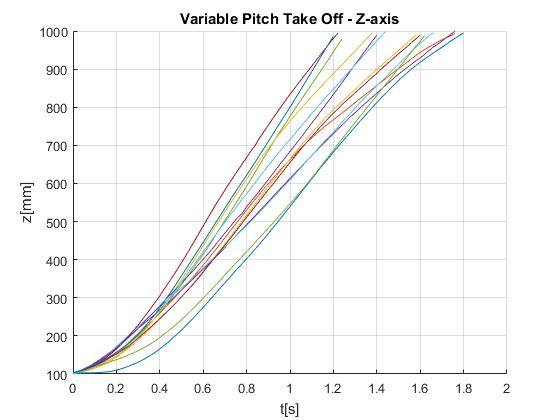
\includegraphics[width = \textwidth, angle= 0]{VAPIQ-PICTURES/vanjaVPQ}
                        \caption{Movement in z-axis for VPQ}
                    \label{fig:ddoo}
        \end{minipage}
                 \hfill
         \begin{minipage}[b]{0.49\textwidth}
                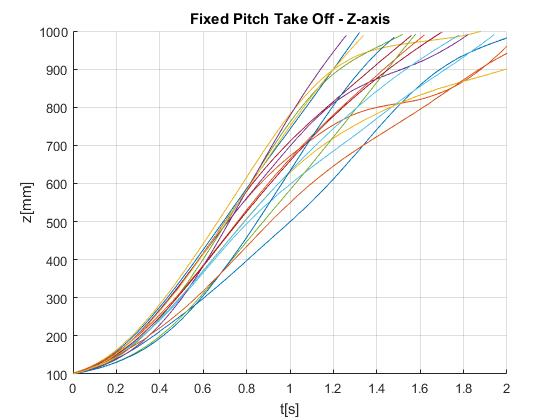
\includegraphics[width = \textwidth, angle =0]{VAPIQ-PICTURES/VanjaFPQ}
                  \caption{Movement in z-axis for FPQ}
                \label{fig:ooaa}
         \end{minipage}
\end{figure}

\begin{table}[H]
\caption{Datasets for FPQ and VPQ}
\label{tab:resp}
\centering
\begin{tabular}{| c | c |} 
 \hline
  VPQ  & FPQ \\
 \hline
 1.7600	&    2.0600  \\
 1.7600	&    2.0600  \\
 1.5800	&    1.8800  \\
 1.7600	&    1.8200  \\
 1.2400	&    1.5200  \\
 1.6600	&    1.9400  \\
 1.2200	&    1.5600  \\
 1.8000	&    1.3200  \\
 1.3800	&    1.6200  \\
 1.3800	&    2.4200  \\
 1.4000	&    1.2600  \\
 1.6200	&    1.5800  \\
 1.4400	&    1.7800  \\
 1.6000	&    1.7000  \\
 1.2000	&    1.4800  \\
    	&    2.2000  \\
	    &    1.3400  \\
\hline
\end{tabular}
\end{table}
\begin{table}[H]
\caption{Table of Data}
\label{tab:infooos}
\centering
\begin{tabular}{| c | c |c| c|} 
  \hline
  Quadcopter Dataset & Mean & Standard Deviation & Number of samples \\
 \hline
 VPQ & 1.5200 & 0.2107   & 15 \\
 FPQ & 1.7376 & 0.3262   & 17\\
 \hline
\end{tabular}
\end{table}

From the information obtained from Tab. \ref{tab:infooos} the following calculations can be conducted:

\begin{equation}
\label{eq:intvar}
S^2_P=\frac{(n_1-1)S^2_1+(n_2-1)S^2_2}{n_1+n_2-2}=S^2_P=\frac{(15-1)\cdot0.2107^2+(17-1)\cdot0.3262^2}{15+17-2}=0.0775
\end{equation}\bigskip

Eq. \ref{eq:intvar} determines the pooled variance, which is used in Eq. \ref{eq:T1}. The similarity of the means from the two datasets are tested based on the test observer T (t-test). The test observer T is determined by:\\
\begin{equation}
\label{eq:T1}
  T = \frac{\overline{VPQ} - \overline{FPQ}}{\sqrt{\frac{S_P^2}{n_1}+\frac{S_P^2}{n_2}}} = \frac{1.5200-1.7376}{\sqrt{ \frac{0.0775}{15}+\frac{0.0775}{17} }} = -2.207
\end{equation}\bigskip

When considering whether or not the null hypothesis shall be discarded, the level of significance must be determined, based on the level of rejection error that can be accepted. It is normal to choose a level of significance, $\alpha= 0.05$. \bigskip

The degrees of freedom are determined by the size of the datasets. In this case, the degrees of freedom are determined by: 
\begin{equation}
\label{eq:dofd}
n_1+n_2-2 = 15 + 17 - 2 = 30
\end{equation}

Based on the calculated T-observer, the chosen significance level and the calculated degrees of freedom, the null hypothesis is discarded if $|T|>t_{\frac{\alpha}{2}}$. \bigskip

In Eq. \ref{eq:disc1} the value of $t_{\alpha}$ is determined by the T-distribution Quantum table in \cite{statistikk}. 

\begin{equation}
\label{eq:disc1}
|T|>t_{\frac{\alpha}{2}} = |T|>t_{\frac{0.05}{2}} = |T|>t_{0.025} = |T|>t_{0.025} = |T|>2.042
\end{equation}

Eq. \ref{eq:res2} shows that the absolute value of T is larger than the the critical value $t_{\alpha}$. 
\begin{equation}
\label{eq:res2}
   2.207>2.042
\end{equation}

Tab.\ref{tab:ttesft} displays the T-test performed in Excel. Excel also determined the same value of T as in Eq. \ref{eq:T1}.  

\begin{table}[H]
\caption{T-Test from Excel}
\label{tab:ttesft}
\centering
\begin{tabular}{| l | c | c |} 
  \hline
  & VPQ & FPQ\\
 \hline
 Mean & 1.5200 & 1.7376. \\
 Observations & 15 & 17 \\
 \hline
 Degrees of freedom & 30 &  \\
 t-stat (T) & -2.2070 & \\
 T-critical & 2.0423 & \\
 \hline
\end{tabular}
\end{table}\bigskip

Based on these calculations, the null hypothesis is rejected. This means that there is a significant difference between the response time for variable pitch and fixed pitch propellers. 
\newpage


%%%%%%%%%%%%%%%%%%%%%%%%%%%%%%%%%%%%%%%%%%%%%%%%%
%%%%%%%%%%%%%%%%%%%%%%%%%%%%%%%%%%%%%%%%%%%%%%%%%

\section{Variable Pitch Motor RPM}
To determine the RPM of the motor produced relative to the combination of PWM and pitch angle, a stroboscope was used.

\subsection{\textsc{\medium Test Setup}}
A stroboscope was used to determine the RPM of the AXI motor with the Model Motors variable pitch mechanism. The quadcopter was fastened to the ground with software that did not affect the PID-controller. A combination of PWM and pitch values were tested and the RPM value was determined by manually adjusting the stroboscope while the motor and propeller rotated. 

\subsection{\textsc{\medium Test Assessment}}
The pitch angle has an impact on the measured RPM value, a higher pitch value gives a lower RPM. A linear increment in throttle does not give a linear output in rotational speed. It was observed during this test that when the PWM value was increased, based upon throttle input, it resembled a sine curve. Therefore, the motor appears to be more sensitive with throttle values close to PWM around 1000 and PWM around 2000, and less sensitive around 1300 to 1700 PWM. The test can be done with a various amount of combination of pitch and PWM, this has not been done for the whole plane.

\subsection{\textsc{\medium Test Results}}
Tab. \ref{tab:rpm1} shows the RPM values measured with the stroboscope when the quadcopter ran on the standard flight values. The standard flight values for pitch versus PWM are the ones used for all flight tests.
\begin{table}[H]
\caption{Standard Parameters}
\label{tab:rpm1}
\centering
\begin{tabular}{| c | c | c |} 
  \hline
 PWM & Pitch & Measured RPM\\
 \hline
 1300 & 0 & 8000 \\
 1425 & 8-9 & 10600 \\
 1550 & 18 & 11000 \\
 \hline
\end{tabular}
\end{table}\bigskip

While determining the the appropriate parameters for the flight tests, it emerged that the quadcopter needed to have a PWM value above 1750 to not be affected by the resonance frequency. Tab. \ref{tab:rpm2} displays the RPM values obtained when the same test was ran on the determined critical speed.

\begin{table}[H]
\caption{Critical Speed 1}
\label{tab:rpm2}
\centering
\begin{tabular}{| c | c | c |} 
  \hline
 PWM & Pitch & Measured RPM\\
 \hline
 1750 & 0 & 12000 \\
 1875 & 8-9 & 12500 \\
 2000 & 18 & Stall \\
 \hline
\end{tabular}
\end{table}\bigskip

Tab. \ref{tab:rpm2} shows that when the motor received a PWM value of 2000, and the pitch was set to approximately 18 degrees, the motor stalled. When a motor stalls it means that it experiences a higher load than it is designed for. Therefore, it can no longer supply enough torque to keep the motor spinning. The maximum pitch angle was decreased to 10 degrees. The RPM values measured relating to the PWM and pitch, when the maximum pitch was decreased, are displayed in Tab. \ref{tab:rpm3}.

\begin{table}[H]
\caption{Critical Speed 2}
\label{tab:rpm3}
\centering
\begin{tabular}{| c | c | c |} 
  \hline
 PWM & Pitch & Measured RPM\\
 \hline
 1750 & 0 & 12100 \\
 1875 & 4-5 & 13000 \\
 2000 & 10 & 15500 \\
 \hline
\end{tabular}
\end{table}\bigskip

During these tests the implemented compensation in throttle was discovered to be sub optimal. The reason for this is that the pitch and RPM are increased based upon the same throttle input. This means that increasing the throttle gives a linear increase in thrust and pitch. However the greater the pitch value the higher compensation of RPM is required. \bigskip
Based on the results obtained, Eq. \ref{eq:ligning} was determined.
\begin{equation}
\label{eq:ligning}
y = 8.227x_1 + 56.246x_2 -2425.748
\end{equation}\bigskip
The equation is a multiple linear regression equation, given as \begin{center}$y = a + b_1*x_1 + b_2*x_2$. \\ \end{center}
Where y is the RPM, x1 is the throttle input and x2 is the pitch angle. By using the Eq. \ref{eq:ligning}, the RPM value should be closer to constant based upon the throttle input and pitch angle. The coefficient of determination is 0.91 A multiple nonlinear regression model would be better, but no feasible model was found due to little test data. 





%%%%%%%%%%%%%%%%%%%%%%%%%%%%%%%%%%%%%%%
%%%%%%%%%%%%%%%%%%%%%%%%%%%%%%%%%%%%%%%
%%%%%%%%%%%%%%%%%%%%%%%%%%%%%%%%%%%%%%%
%%%%%%%%%%%%%%%%%%%%%%%%%%%%%%%%%%%%%%%
\begin{comment}
\section{Ground Effect}
%%%%%%%%%%%%%%%%%%%%%%%
$H_0$ = A Quadcopter with variable pitch propellers can \\
$H_1$ = A Quadcopter with variable pitch propellers can not 
\\\\
%%%%%%%%%%%%%%%%%%%%%%%%%%%%%%%%%%%%%%%
\begin {table}[H]
    \begin{center}
    \caption {Target Position} 
    \label{tab:bla} 
    \begin{tabular}{|l|l|}\hline 
        \textbf{Color:}    & \textbf{Radius [mm]:} \\ \hline
        Green   &  $<$ 25 \\ \hline
        Light Green & $<$ 50 \\\hline
        Yellow & $<$ 75 \\ \hline
        Orange & $<$ 100 \\ \hline
        Red    & $<$ 125 \\ \hline
        Other  & $>$ 150 \\ \hline
        \end{tabular}
    \end{center}
\end{table}

\section{Hover}
    
    http://stattrek.com/hypothesis-test/difference-in-means.aspx?Tutorial=AP
    
    %%%%%%%%%%%%%%%%%%%%%%%
    $H_0$ = A Quadcopter with variable pitch propellers can \\
    $H_1$ = A Quadcopter with variable pitch propellers can not 
    \\\\
    %%%%%%%%%%%%%%%%%%%%%%%%%%%%%%%%%%%%%%%
    histogram
    lager 
    30 stk
    http://www.mn.uio.no/ibv/tjenester/kunnskap/plantefys/matematikk/stat.html#zscore
    %%%%%%%%%%% LOOP 800
    Loop 800 is a measure of the time it takes a propulsion system to increase thrust from 100g to 800g and then decelerate to 400g. It is used to measure the responsiveness of a propulsion system. 
    $H_0$ = A Quadcopter with variable pitch propellers can \\  
    $H_1$ = A Quadcopter with variable pitch propellers can not 
    \\\\
    normaltestplott
    z-axis up and down
    ground effect
    Signifikansnivå?
\end{comment}